\documentclass[../text.tex]{subfiles} 

\begin{document}


\section{Collar--gluings and Factorization Algebras}\label{ch:gluing_disk_alg}

Given a stratified manifold $M$, and a $\otimes$-presentable $\infty$-category $\catC$, we defined the $\infty$-category $\lcfa_M (\catC)$ of locally constant factorization algebras on $M$ valued in $\catC$. We also noticed, in \Cref{thm:disk_alg=lcfa}, that factorization homology is involved in constructing these algebras from local data. This prompts us to ask if we can say something about the behavior of this $\infty$-category under collar--gluings in the manifold variable. In this section we will prove that such a result exists in both the cases of locally constant and ordinary factorization algebras.


\subsection{The Gluing Theorem}

\begin{theorem}\label{thm:gluing_lcfas}
    Given a collar-gluing of stratified manifolds $f: M \rightarrow [-1,1]$, the $\infty$-category of $\disk_{/M}$-algebras is equivalent to the pullback of $\infty$-categories
    %
    \begin{equation}
        \lcfa_M (\catC) \simeq \lcfa_{M_-} (\catC) \bigtimes_{\lcfa_{M_0 \times \mathbb{R}} (\catC)} \lcfa_{M_+}(\catC).
    \end{equation}
\end{theorem}

As in previous cases the proof of the above theorem will have a corollary that is easier to prove and whose proof goes along the same lines

\begin{corollary}\label{cor:gluing_falgs}
    A collar-gluing of stratified manifolds $f: M \rightarrow [-1,1]$ induces an equivalence of $\infty$-categories
    %
    \begin{equation}
        \falg_M (\catC) \simeq \falg_{M_-} (\catC) \bigtimes_{\falg_{M_0 \times \mathbb{R}} (\catC)} \falg_{M_+}(\catC).
    \end{equation}
\end{corollary}

Before me move on to the proof of the above two results we pause to record a few useful lemmas that will play a role in it.

\begin{lemma}\label{lem:fbar_func}
    A collar-gluing $f:M \xrightarrow{} [-1,1]$ of a stratified manifold $M$ induces a functor
    %
    \begin{equation}
        \bar{f}: \mfld[r]_{/M} \xrightarrow{\ \ \ \ } \alg{\mathsf{Assoc^{RL}}} (\mfld[r]_{/M}),
    \end{equation}
    %
    which on objects acts as $(N \xhookrightarrow{} M) \mapsto (N_- \xhookrightarrow{} M, N_0 \times \mathbb{R} \xhookrightarrow{} M, N_+ \xhookrightarrow{} M)$.
\end{lemma}

\begin{proof}
    We recall that the underlying $\infty$-category of $\mfld[r]_{/M}$ is actually (the nerve of) an ordinary category. In particular, morphisms are given by the data of an embedding $N \xhookrightarrow{} N'$ such that $N \xhookrightarrow{} N' \xhookrightarrow{} M = N \xhookrightarrow{} M$ on the nose.
    
    A collar-gluing of $M$ restricts to a collar-gluing of any $N$ that has an embedding into $M$ like the objects of our category. On the right-hand side, at the level of objects, the associative algebra structure is provided by embeddings that differ in the $\mathbb{R}$ factor and the module maps are provided by embeddings of the middle $N_0 \times \mathbb{R}$ into $N_-$ and $N_+$. At the level of morphisms we send the morphism $e: N \xhookrightarrow{} N'$ to
    %
    \begin{equation}
        (e_-: N_- \xhookrightarrow{} N'_-, \ e_0: N_0 \times \mathbb{R} \xhookrightarrow{} N'_0 \times \mathbb{R}, \ e_+: N_+ \xhookrightarrow{} N'_+).
    \end{equation}
    %
    The existence of these maps can be stated as the existence of a unique factorization, as in e.g.
    %
    \begin{equation}\label{cd:factorization_of_e}
        \begin{tikzcd}
            N_- \arrow[r, hook] \arrow[rd, dashed, hook, "e_-"'] & N \arrow[r, hook, "e"] & N', \\
            & N'_- \arrow[ru, hook] &
        \end{tikzcd}
    \end{equation}
    %
    where the diagram commutes on the nose. Such an assignment clearly plays well with the algebra structure of the right-hand side, through the existence of (on the nose) commutative diagrams like e.g.
    %
    \begin{equation}
        \begin{tikzcd}
            N_0 \times \mathbb{R} \arrow[r, hook, "e_0"] \arrow[d, hook] & N'_0 \times \mathbb{R} \arrow[d, hook]\\
            N_- \arrow[r, hook, "e_-"] & N'_-,
            \end{tikzcd}
    \end{equation}
    %
    so that we clearly get a functor
    %
    \begin{equation}
        \bar{f}: \mfld[r]_{/M} \xrightarrow{\ \ \ \ } \alg{\mathsf{Assoc^{RL}}} (\mfld[r]_{/M}).
    \end{equation}
\end{proof}

\begin{remark}
    In the above lemma it is important that we stuck to the comparatively simple $\mfld[r]_{/M}$ instead of $\mfld_{/M}$. It is not immediately obvious how to deal with the higher morphisms in the latter, as can be seen from the form of \Cref{cd:factorization_of_e}. The issues are related to the ones that appear in the construction of the pushforward functor \Cref{thm:fh_pushforward}. A simple case to ponder is an isotopy that maps one embedding of a disk in $M_- \setminus (M_0 \times \mathbb{R})$ to another one in $M_+ \setminus (M_0 \times \mathbb{R})$.
\end{remark}

\begin{lemma}\label{lem:B_sym_mon}
    The bar construction $\mathsf{B}: \alg{\mathsf{Assoc^{RL}}} (\catC) \xrightarrow{\ \ } \catC$ is a symmetric monoidal functor.
\end{lemma}

\begin{proof}
    The symmetric monoidal structure of $\alg{\mathsf{Assoc^{RL}}} (\catC)$ is inherited from $\catC$ pointwise. We denote the objects of $\alg{\mathsf{Assoc^{RL}}} (\catC)$ as $(R,A,L)$, and use $\mathsf{B}_{\bullet} (R, A, L):\Delta^{\mathsf{op}} \rightarrow \catC$ for the simplicial object of the bar construction. Using the language of \cite[def.2.1.2.7]{lurie_ha}, to prove that $\mathsf{B}$ is symmetric monoidal amounts to showing that for each basepoint--preserving map of based finite sets $f: I_* \xrightarrow{} J_*$ there is a commutative diagram of $\infty$-categories
    %
    \begin{equation}
        \begin{tikzcd}
            \alg{\mathsf{Assoc^{RL}}} (\catC)^I \arrow[r, "\mathsf{B}^I"] \arrow[d, "f_*"] & \catC^I \arrow[d, "f_*"] \\
            \alg{\mathsf{Assoc^{RL}}} (\catC)^J \arrow[r, "\mathsf{B}^J"] & \catC^J.
        \end{tikzcd}
    \end{equation}
    
    Following \cite[rem.2.1.2.2]{lurie_ha}, each $f$ admits a unique factorization as a composition of an active and an inert map. We can also further uniquely decompose the active maps into surjective active maps and injective active maps. So we will examine the above for each type of map separately. The case of inert maps is trivial as always, because of the simplicity of $f_*$. The case of injective active maps is essentially guaranteeing that $\mathsf{B}$ maps the monoidal unit to the monoidal unit. In this case the existence of the commutative diagram is provided by
    %
    \begin{equation}
        \mathsf{B} (\mathbb{1}_{\alg{\mathsf{Assoc^{RL}}} (\catC)}) = \mathsf{colim} (\mathsf{B}_{\bullet} (\mathbb{1},\mathbb{1},\mathbb{1})) \simeq \mathsf{colim} (\Delta^{\mathsf{op}} \xrightarrow{\{ \mathbb{1}\}} \catC) \simeq \mathbb{1}.
    \end{equation}
    %
    Finally, the case of surjective active morphisms describes what happens when we use the monoidal product to multiply. In this case we will look at the model calculation for the active map $f: \langle 2 \rangle \xrightarrow{} \langle 1 \rangle$. All other possibilities go along similar lines. Given two objects $H = (R,A,L)$ and $H' = (R',A',L')$ we have 
    %
    \begin{align}
        \mathsf{B}(H \otimes H') &= \mathsf{colim} (\mathsf{B}_{\bullet} ((R,A,L) \otimes (R',A',L')))\notag\\
        &= \mathsf{colim} (\mathsf{B}_{\bullet} (R \otimes R', A \otimes A', L \otimes L'))\notag\\
        &\simeq \mathsf{colim} (\mathsf{B}_{\bullet} (R, A, L) \otimes \mathsf{B}_{\bullet} (R', A', L'))\notag\\
        &= \mathsf{colim} (\Delta^{\mathsf{op}} \rightarrow \Delta^{\mathsf{op}} \times \Delta^{\mathsf{op}} \xrightarrow{\mathsf{B}_{\bullet} (R, A, L) \otimes \mathsf{B}_{*} (R', A', L')} \catC)\notag\\
        &\simeq \mathsf{colim} (\Delta^{\mathsf{op}} \times \Delta^{\mathsf{op}} \xrightarrow{\mathsf{B}_{\bullet} (R, A, L) \otimes \mathsf{B}_{*} (R', A', L')} \catC)\notag\\
        &\simeq \mathsf{colim} (\mathsf{B}_{\bullet} (R, A, L)) \otimes \mathsf{colim} (\mathsf{B}_{*} (R', A', L'))\notag\\
        &= \mathsf{B}(H) \otimes \mathsf{B}(H'),
    \end{align}
    %
    where $\Delta^{\mathsf{op}} \rightarrow \Delta^{\mathsf{op}} \times \Delta^{\mathsf{op}}$ is the diagonal functor. The first equivalence comes from the symmetric monoidal structure of $\catC$ dues to reshuffling in the simplicial object. The second equivalence uses the finality of the diagonal functor which comes from the fact that $\Delta^{\mathsf{op}}$ is sifted. Finally, the third equivalence exists because the symmetric monoidal structure of $\catC$ commutes with (sifted) colimits.
\end{proof}

\begin{proof}[Proof of \Cref{cor:gluing_falgs}]
    We will first focus on the case of factorization algebras and prove the statement of \Cref{cor:gluing_falgs}. Moreover, because of \Cref{cor:disk_alg=falg}, this means that we will focus on $\disk[r]_{/M}$-algebras.
    
    The data of a collar-gluing provides open embeddings $M_0 \times \mathbb{R} \xhookrightarrow{} M_-$ and $M_0 \times \mathbb{R} \xhookrightarrow{} M_+$, where $M_-$, $M_0$ and $M_+$ have the usual meanings as in \Cref{def:collar-gluing}. This can be used to construct the cospan of restriction functors $\alg{\disk[r]_{/M_-}} (\catC) \rightarrow \alg{\disk[r]_{/M_0 \times \mathbb{R}}} (\catC) \leftarrow \alg{\disk[r]_{/M_+}} (\catC)$. Using this data we can define the pullback $\infty$-category
    %
    \begin{equation}
        \mathscr{P} := \alg{\disk[r]_{/M_-}} (\catC) \bigtimes_{\alg{\disk[r]_{/M_0 \times \mathbb{R}}} (\catC)} \alg{\disk[r]_{/M_+}} (\catC).
    \end{equation}
    %
    The further open embeddings of $M_-$, $M_0 \times \mathbb{R}$ and $M_+$ into $M$ again give rise to restriction functors that form a(n on the nose) commutative square
    %
    \begin{equation}
        \begin{tikzcd}
            \alg{\disk[r]_{/M}} (\catC) \arrow[r] \arrow[d] & \alg{\disk[r]_{/M_+}} (\catC) \arrow[d] \\
            \alg{\disk[r]_{/M_-}} (\catC) \arrow[r] & \alg{\disk[r]_{/M_0 \times \mathbb{R}}} (\catC),
        \end{tikzcd}
    \end{equation}
    %
    which, by the universal property of the pullback, gives us a canonical functor $\rho: \alg{\disk[r]_{/M}} (\catC) \rightarrow \mathscr{P}$. Our job is to find an inverse to this functor.
    
    Consider the following construction. Given the data of an object $(A_-, A_+) \in \alg{\disk[r]_{/M_-}} (\catC) \times \alg{\disk[r]_{/M_+}} (\catC)$ such that $A_-|_{M_0 \times \mathbb{R}} = A_+|_{M_0 \times \mathbb{R}} = : A_0$ we want to construct a functor $A: \disk[r]_{/M} \xrightarrow{} \catC$. We do this by relying on factorization homology and the bar construction. Given $(U \xhookrightarrow{} M) \in \disk[r]_{/M}$ we define
    %
    \begin{equation}\label{eq:def_of_A_in_proof}
        A(U) := \int_{U_-} A_- \bigotimes\limits_{\int_{U_0 \times \mathbb{R}} A_0} \int_{U_+} A_+,
    \end{equation}
    %
    where $U_-$, $U_0$ and $U_+$ are defined through the inherited collar-gluing $U \xhookrightarrow{} M \xrightarrow{} [-1,1]$. Well-definition of the bar construction is provided if we have the appropriate left and right module structures on $\int_{U_-} A_-$ and $\int_{U_+} A_+$ over the associative algebra $\int_{U_0 \times \mathbb{R}} A_0$. Pushforward along the restrictions $f|_{U_-}: U_- \rightarrow \left[-1, 1\right)$ and $f|_{U_+}: U_+ \rightarrow \left(-1, 1\right]$, together with the properties of factorization homology provides these left and right module structures. Furthermore, the associative algebra object is exactly the appropriate one since consecutive restrictions commute on the nose. The above argument is essentially the statement that there is a functor
    %
    \begin{align}
        \gamma: \mathscr{P} \xrightarrow{\ \ \int \ \ } &\alg{\mfld[r]_{/M_-}}(\catC) \bigtimes\limits_{\alg{\mfld[r]_{/M_0 \times \mathbb{R}}} (\catC)} \alg{\mfld[r]_{/M_+}} (\catC)\notag\\ &\xrightarrow{\ - \circ \bar{f} \ } \mathsf{Fun}(\mfld[r]_{/M}, \alg{\mathsf{Assoc^{RL}}} (\catC)) \xrightarrow{\ \mathsf{B} \circ - \ } \mathsf{Fun}(\mfld[r]_{/M},\catC) \xrightarrow{\ } \mathsf{Fun}(\disk[r]_{/M}, \catC),
    \end{align}
    %
    where $\bar{f}$ is the functor from \Cref{lem:fbar_func}.

    Our first order of business is to show that $\gamma$ actually even lands in $\alg{\disk[r]_{/M}} (\catC)$, and not just $\mathsf{Fun}(\disk[r]_{/M}, \catC)$. Since we have expressed the construction $A = \gamma(A_-, A_+)$ functorially, we can see that $A$ will inherit the structure of an algebra from the fact that factorization homology and the bar construction are symmetric monoidal functors (see \Cref{lem:B_sym_mon} for the latter), together with \Cref{lem:fbar_func} that lends this property to $\bar{f}$. With that we have constructed a functor
    %
    \begin{equation}
        \gamma : \mathscr{P} \xrightarrow{\ \ \ \ } \alg{\disk[r]_{/M}} (\catC).
    \end{equation}
    
    Or strategy will be to show that the pair of functors $\rho$ and $\gamma$ give rise to an equivalence by first checking that this is the case on maximal $\infty$-subgroupoids and subsequently that it is also so on morphism spaces. Towards the first goal we need to show that:
    %
    \begin{enumerate}
        \item $\rho( \gamma (A_-, A_+))$ reproduces $(A_-, A_+)$ up to equivalence, and
        \item $\gamma (\rho (A))$ reproduces $A$ up to equivalence.
    \end{enumerate}
    %
    We now check these in order. Checking (1) amounts to evaluating disks $U$ which are contained in only one of the pieces $M_-$, $M_0 \times \mathbb{R}$ and $M_+$. For the case of $U_0 \times \mathbb{R} = \emptyset = U_+$, we have
    %
    \begin{equation}
        A(U) = \int_{U} A_- \bigotimes\limits_{\mathbb{1}} \mathbb{1} \simeq A_- (U),
    \end{equation}
    %
    and similarly if $U_- = \emptyset = U_0 \times \mathbb{R}$. Alternatively, for the case of $U_- = U_0 \times \mathbb{R} = U_+$ we instead have
    %
    \begin{equation}
        A(U) = \int_U A_0 \bigotimes\limits_{\int_{U} A_0} \int_U A_0 \simeq A_0(U).
    \end{equation}
    %
    If $U$ is such that $U_+ = \emptyset$, but $U_0 \times \mathbb{R} \neq \emptyset$ then
    %
    \begin{equation}
        A(U) = \int_U A_- \bigotimes\limits_{\int_{U_0 \times \mathbb{R}} A_-} \mathbb{1} \simeq \int_U A_- \bigotimes\limits_{\int_{U_0 \times \mathbb{R}} A_-} \int_{\emptyset} A_- \simeq \int_{U} A_- = A_-(U),
    \end{equation}
    %
    where the last equivalence is provided by the collar-gluing property of factorization homology. This observation is also what confirms (2). Namely,
    %
    \begin{equation}
        \int_U A \simeq \int_{U_-} A \bigotimes\limits_{\int_{U_0 \times \mathbb{R}} A} \int_{U_+} A \simeq \int_{U_-} A_- \bigotimes\limits_{\int_{U_0 \times \mathbb{R}} A_0} \int_{U_+} A_+,
    \end{equation}
    %
    where the first equivalence comes from collar-gluing, while the second is a rewriting using the fact that restricting the algebra doesn't change the value of factorization homology it just changes what we can evaluate with it.

    Finally, we want to show that $\rho$ is fully faithful, i.e. we want to show that
    %
    \begin{equation}
        \begin{tikzcd}
            \mathsf{Hom}_{\alg{\disk[r]_{/M}} (\catC)}(A, B) \arrow[r, bend left=4, "\rho"] & \mathsf{Hom}_{\mathscr{P}}((A_-, A_+), (B_-, B_+)) \arrow[l, bend left=4, "\gamma"]
        \end{tikzcd}
    \end{equation}
    %
    represents an equivalence of spaces for each $A, B \in \alg{\disk[r]_{/M}} (\catC)$. That is, we have to do similar computations as (1) and (2) above, but now on the level of morphisms. Nothing new happens in the calculations involving restrictions that don't involve multiple pieces, since their logic essentially only depends on the properties of the bar construction when restricting. In the rest of the calculations we crucially used the collar-gluing property of factorization homology. That this property continues to hold at the morphism level is a consequence of the fact that we made sure to elevate the statement of \Cref{prop:barconst=intinterval} to the level of functors, together with the pushforward property which also holds functorially à la \Cref{rem:fh_pushforward_functorial}. Namely, these provide equivalences of functors
    %
    \begin{equation}
        \int_U - \simeq \int_{[-1,1]} (f|_U)_* - \simeq \mathsf{B} \circ (f|_U)_* = \int_{U_-} (-)_- \bigotimes\limits_{\int_{U_0 \times \mathbb{R}} (-)_0} \int_{U_+} (-)_+,
    \end{equation}
    %
    which is exactly the collar-gluing property extended to the level of morphisms. This shows the equivalence at the level of factorization algebras.
\end{proof}

\begin{proof}[Proof of \Cref{thm:gluing_lcfas}]
    In the case that all $\infty$-categories involved are locally constant we will extend the previous proof to provide the equivalence. Since we know that restriction does not destroy local constancy, extending the result to the case of locally constant factorization algebras simply requires us to show that the gluing $\gamma$ also preserves this property. Let $U \xhookrightarrow{} V$ be two disks of $M$. What we have to check is that there is an equivalence
    %
    \begin{equation}
        \int_U \gamma(A_-, A_+) \xrightarrow{\ \ \simeq \ \ } \int_V \gamma(A_-, A_+)
    \end{equation}
    %
    in $\catC$. We will achieve this if we find compatible equivalences,
    %
    \begin{align}
        &\int_{U_-} A_- \simeq \int_{V_-} A_-& &\int_{U_0 \times \mathbb{R}} A_0 \simeq \int_{V_0 \times \mathbb{R}} A_0& &\int_{U_+} A_+ \simeq \int_{V_+} A_+,&
    \end{align}
    %
    on each of the pieces $(U_- \xhookrightarrow{} V_-), (U_0 \times \mathbb{R} \xhookrightarrow{} V_0 \times \mathbb{R}), (U_+ \xhookrightarrow{} V_+)$, and combine them using the bar construction. If these pieces were disks then the above equivalences would be given by the local constancy of the constituent locally constant factorization algebras.
    
    Generically though, these pieces will not be disks again, so we can't simply inherit the local constancy property immediately. To alleviate this issue we make use of \Cref{thm:decom_strat_man} which assures us that every manifold can be obtained by collar--gluings and sequential colimits if we start with disks. In fact, since our largest manifold of interest is a disk, which is finitary, we only need collar--gluings, and not sequential colimits. Thus, we can work inductively and iterate the cutting and gluing process until the pieces become disks. The only thing that we need to check is that through one inductive step the equivalences remain compatible.
    
    Specifically, by compatibility here we mean that there is a commutative diagram
    %
    \begin{equation}\label{cd:equivs_from_lc}
        \begin{tikzcd}
            \int_{U_-} A_- \arrow[d, "\simeq"] & \int_{U_0 \times \mathbb{R}} A_0 \arrow[d, "\simeq"] \arrow[l] \arrow[r] & \int_{U_+} A_+ \arrow[d, "\simeq"] \\
            \int_{V_-} A_- & \int_{V_0 \times \mathbb{R}} A_0 \arrow[l] \arrow[r] & \int_{V_+} A_+,
        \end{tikzcd}
    \end{equation}
    %
    where the horizontal arrows are induced by the relevant embeddings. A sufficient condition to guarantee compatibility is that all collar--gluings are defined as collar--gluings of $M$ and then inherited to every open submanifold through its embedding in $M$. Focusing on the final two consecutive collar--gluings we get a commutative diagram, which we schematically denote
    %
    \begin{equation}
        \begin{tikzcd}
            -+ & 0+ \arrow[l] \arrow[r] & ++\\
            -0 \arrow[u] \arrow[d] & 00 \arrow[u] \arrow[l] \arrow[r] \arrow[d] & +0 \arrow[d] \arrow[u] \\
            -- & 0- \arrow[l] \arrow[r] & +-,
        \end{tikzcd}
    \end{equation}
    %
    one for each of $U$ and $V$. Stacking these two with the equivalence as connecting arrows is again a commutative diagram. This is enough information to guarantee that after acting with the bar construction in one direction we again get compatible equivalences. The key point being that we consider the collar--gluings on all pieces in both orders to get all the necessary arrows.

    \begin{multicols}{2}
        \begin{figure}[H]
            \centering
            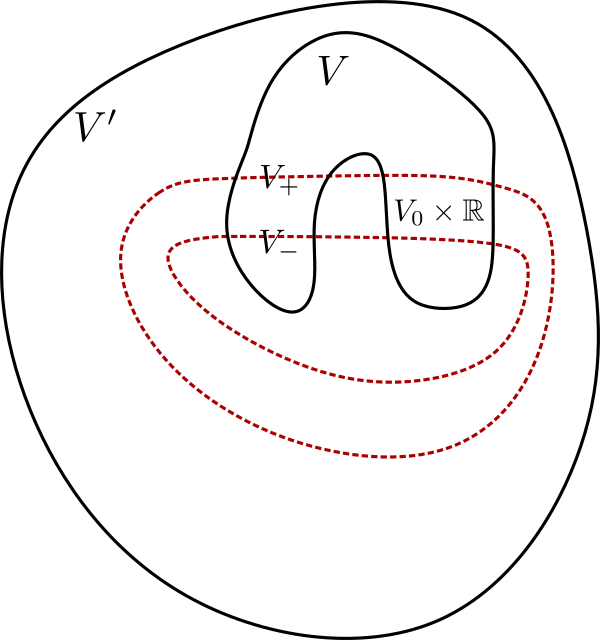
\includegraphics[width=5cm]{../images/extend_gluing.png}
            \caption{Extending a collar-gluing.}
            \label{fig:extend_gluing}
        \end{figure}
        %
        The final point to check is that we have not limited ourselves by insisting to only consider collar--gluings which are inherited from ones on $M$. This is best shown in \Cref{fig:extend_gluing}. Namely, given the disk $V \xhookrightarrow{} M$, we can take a larger disk $V'$, which is guaranteed to exist from the fact that $M$ is a manifold. The figure then shows that given any collar-gluing of $V$ how we can find one particular collar-gluing of $M$ that extends the one of $V$. Since $V'$ is a disk, the figure does not obscure any detail.
    \end{multicols}
\end{proof}

\begin{remark}
    The simple case when the collar-gluing is a disjoint union, and the manifolds are smooth can also be found as \cite[ex.5.4.5.4]{lurie_ha}.
\end{remark}


\subsection{An Outside View of Factorization Algebras}

After the results of the previous section we remark on a general view that we can take for the $\infty$-categories of (locally constant) factorization algebras. Namely, we notice factorization algebras can be cast as a functor
%
\begin{equation}
    \falg_{-}(\catC), \lcfa_{-}(\catC): \mfld[r] \xrightarrow{\ \ \ \ } \cat^{\mathsf{op}},
\end{equation}
%
where the action on morphisms is given by restriction, which is what gives rise to the $^{\mathsf{op}}$. In the case of disjoint union, \Cref{thm:gluing_lcfas} and \Cref{cor:gluing_falgs} then provide the equivalences that are needed to make these into symmetric monoidal functors, where the symmetric monoidal product on $\cat^{\mathsf{op}}$ is given by \emph{coproduct}. We emphasize that the domain of these functors, as defined, is $\mfld[r]$; there is no clear way of how to define the above functors so that they have the domain $\mfld$ with the idea of restriction functors as morphisms.

We know from \Cref{thm:decom_strat_man} that any manifold can be constructed from basics by iterated collar--gluings and sequential colimits. Having described what happens to a locally constant factorization algebras under collar--gluings of manifolds, we now turn to sequential colimits. {\color{red} The gluing result has an ordinary (nonhomotopy) limit. Is this also the output of the (co)bar construction?}

\begin{proposition}\label{prop:fa_seq_col}
    The functors $\falg(\catC)$ and $\lcfa(\catC)$ respect sequential colimits.
\end{proposition}

\begin{proof}
    Using \Cref{thm:disk_alg=lcfa} and \Cref{cor:disk_alg=falg} we will argue in terms of algebras over $\infty$-operads. Since the formation of algebras is contravariantly functorial (as precomposition), it is sufficient to show that there is an equivalence of $\infty$-operads
    %
    \begin{equation}
        \mathsf{colim}_{i \geq 0} \disk_{/M_i} \xrightarrow{\ \ \simeq \ \ } \disk_{M},
    \end{equation}
    %
    as well as the same for $\disk[r]_{/M}$. In the case of the former, as originally noted in the proof of \cite[cor.2.40]{aft_fhstrat}, the result follows from using \cite[cor.1.6.]{dugger2004hypercovers}, an argument about configuration spaces, as well as \cite[lem.2.21]{aft_fhstrat}, which explains the relation of these to the above operad. %In the case of the latter, the situation is even simpler because of its discrete nature. One way to show this is to notice that the functor from the ordinary, nonhomtopy colimit factors through $\mathsf{colim}_{i \geq 0} \disk[r]_{/M_i} \xrightarrow{} \disk[r]_{/M}$, in which case it suffices to find an equivalence of \emph{ordinary} categories
    %
    %\begin{equation}
    %    \mathsf{colim}_{i \geq 0} \disk[r]_{/M_i} \xrightarrow{} \disk[r]_{/M},
    %\end{equation}
    %
    %where the colimit is now the one relevant to ordinary category theory, namely the nonhomotopy one. But it's now easy to see that this the canonical morphism above is an equivalence since for every $U \in \disk_{/M}$ there will be a finite integer $i$, such that $U \subset M_i$.
\end{proof}

With this result we have fully described an algorithm of how to compute the $\infty$-category of factorization algebras on any stratified manifold if we know how to compute it on the basics. Through this algorithm the theory of (locally constant) factorization algebras is fully determined by the assignment
%
\begin{equation}
    U \mapsto \falg_U (\catC),
\end{equation}
%
for each disk $U \in \mathsf{Bsc}$.



\subsection{Some Examples of Gluing}

\begin{example}\label{ex:reproduce_lcfas_on_interval}
    With the ingredients we have introduced up to now, specifically in \Cref{ssec:lcfa_on_ints}, we can do a nontrivial check of the gluing theorem. This is because we can write a collar-gluing of the closed interval $[-1,1] \cong \left[-1,1\right) \coprod_{(-1,1)} \left(-1,1\right] \cong \mathbb{R}_{\geq 0} \coprod_{\mathbb{R}} \mathbb{R}_{\leq 0}$. We note here that we have written $\mathbb{R}_{\leq 0}$ and $\mathbb{R}_{\geq 0}$ to emphasize the maps forming the decomposition. At the level of unstructured objects these two are isomorphic (see also \Cref{rem:left_or_right_module}). For this example, the theorem says that locally constant factorization algebras on the closed interval should be given by
    %
    \begin{equation}
        \lcfa_{[-1,1]} (\catC) \simeq \lcfa_{\mathbb{R}_{\geq 0}} (\catC) \bigtimes_{\lcfa_{\mathbb{R}} (\catC)} \lcfa_{\mathbb{R}_{\leq 0}} (\catC) \simeq \mathsf{RMod} (\catC) \bigtimes_{\alg{\mathbb{E}_1} (\catC)} \mathsf{LMod} (\catC),
    \end{equation}
    %
    where the functors are the ones that forget the module. At the level of objects, this is the data of an algebra with a right module $(A, R) \in \mathsf{RMod} (\catC)$ and an algebra with a left module $(B, L) \in \mathsf{LMod} (\catC)$, such that the algebras are equal $A = B$. But this is exactly the same as the description we gave in terms of an algebra with a left and a right module, i.e. an algebra over $\mathsf{Assoc^{RL}}$, in \Cref{cor:lcfas_on_closed_int}.
\end{example}

\begin{example}\label{ex:reproduce_lcfas_on_S1}
    A highly nontrivial check of the gluing theorem is given by the circle $S^1$. Using results from \cite[prop.4.0.1]{cg2016}, namely inheritance from a covering space, \cite[sec.5.5]{ginot2015} characterizes locally constant factorization algebras on the circle $S^1$ as
    %
    \begin{equation}
        \lcfa_{S^1} (\catC) \simeq \mathsf{Aut} (\alg{\mathbb{E}_1} (\catC)),
    \end{equation}
    %
    i.e. $\mathbb{E}_1$-algebras together with a self-equivalence. This result is not generalizable to higher spheres because it uses the technology of covering spaces. \Cref{thm:gluing_lcfas} allows us to recover this nontrivial result. To wit, the circle can be exhibited as a collar-gluing $S^1 \cong \mathbb{R} \coprod_{S^0 \times \mathbb{R}} \mathbb{R} \cong \mathbb{R} \coprod_{\mathbb{R} \sqcup \mathbb{R}} \mathbb{R}$. For locally constant factorization algebras this means that
    %
    \begin{equation}\label{eq:lcfas_on_S1_gluing}
        \lcfa_{S^1} (\catC) \simeq \lcfa_{\mathbb{R}} (\catC) \bigtimes_{\lcfa_{\mathbb{R} \sqcup \mathbb{R}} (\catC)} \lcfa_{\mathbb{R}} (\catC) \simeq \alg{\mathbb{E}_1} (\catC) \bigtimes_{\lcfa_{\mathbb{R} \sqcup \mathbb{R}} (\catC)} \alg{\mathbb{E}_1} (\catC).
    \end{equation}
    %
    Since a disjoint union is a collar-gluing we also have that $\lcfa_{\mathbb{R} \sqcup \mathbb{R}} \simeq \lcfa_{\mathbb{R}} (\catC) \times \lcfa_{\mathbb{R}} (\catC) \simeq \alg{\mathbb{E}_1} (\catC) \times \alg{\mathbb{E}_1} (\catC)$. Let's denote the restriction functors that restrict to the first and the second component of the disjoint union $\mathbb{R} \sqcup \mathbb{R}$ by $|_1$ and $|_2$ respectively. Going back to \Cref{eq:lcfas_on_S1_gluing}, the data of a locally constant factorization algebra on $S^1$ is equivalent to the data of two $\mathbb{E}_1$-algebras $A$ and $B$ such that their restrictions $A|_1 = B|_1$ and $A|_2 = B|_2$ agree. Since all of these are $\mathbb{E}_1$-algebras there are equivalences with the restrictions forming
    %
    \begin{equation}
        \begin{tikzcd}[row sep = small, column sep= small]
            & A|_1 \arrow[r, phantom, "=", description] & B|_1 & \\
            A \arrow[rd, phantom, "\simeq", sloped, description] \arrow[ru, phantom, "\simeq", sloped, description] & & & B \arrow[lu, phantom, "\simeq", sloped, description] \arrow[ld,  phantom, "\simeq", sloped, description] \\
            & A|_2 \arrow[r, phantom, "=", description] & B|_2 &                        
        \end{tikzcd}
    \end{equation}
    %
    That is we have the data of two algebras $A$ and $B$, and two equivalences from $A$ to $B$. It is standard that this data is equivalent (in one direction by composing) to the data of an $\mathbb{E}_1$-algebra with a self-equivalence.
\end{example}

\begin{example}\label{ex:lcfas_on_S^n}
    Unlike the covering space result for the circle \cite[sec.5.5]{ginot2015} which doesn't generalize to higher spheres, the gluing theorem has no such restriction. Just as for the circle, higher spheres can also be described as a collar-gluing $S^n \cong \mathbb{R}^n \coprod_{S^{n-1} \times \mathbb{R}} \mathbb{R^n}$. Thus, we can iterate the procedure from \Cref{ex:reproduce_lcfas_on_S1} to get the locally constant factorization algebras on all higher spheres. For example, for the two-sphere $S^2$ we have
    %
    \begin{equation}
        \lcfa_{\mathbb{R}^2}(\catC) \bigtimes_{\lcfa_{S^1 \times \mathbb{R}}(\catC)} \lcfa_{\mathbb{R}^2}(\catC) \simeq \alg{\mathbb{E}_2}(\catC) \bigtimes_{\alg{\mathbb{E}_1}( \mathsf{Aut} (\alg{\mathbb{E}_1} (\catC))) } \alg{\mathbb{E}_2} (\catC),
    \end{equation}
    %
    namely, a locally constant factorization algebra on $S^2$ is equivalent to two $\mathbb{E}_2$-algebras, such that they restrict on the fattened equator to the same $\mathbb{E}_2$-algebra equipped with an $\mathbb{E}_1$-automorphism. It is nontrivial to describe this data in a simpler way as was possible for $S^1$.
    
    From this example we can easily see that beyond the dimensionality $n$ of the space, which is locally kept track of as an $\mathbb{E}_n$-algebra, locally constant factorization algebras for the higher spheres also keep track of higher coherent (self-)equivalences, which imitate triangulations of the spheres.
\end{example}

\begin{example}\label{ex:cylinder_mobius_band}
    In \Cref{ch:classif_defect_mfld} we will see that fiber bundles are important for the classification of some stratified manifolds. Here we will look at line bundles over the circle as a toy example, namely, the cylinder $C$ and M\"obius band $M$. The cylinder, as a trivial fiber bundle, is isomorphic to the product space $S^1 \times \mathbb{R}$. By \Cref{prop:exp_of_products_lc} together with the results of \Cref{ex:reproduce_lcfas_on_S1}, locally constant factorization algebras on it are given by $\mathbb{E}_2$-algebras together with an $\mathbb{E}_1$-self-equivalence
    %
    \begin{align}
        \lcfa_C (\catC) \simeq \mathsf{Aut}_{\mathbb{E}_1} (\alg{\mathbb{E}_2} (\catC)).
    \end{align}

    Switching our attention to the M\"obius band $M$, we can use a similar logic as in \Cref{ex:reproduce_lcfas_on_S1} to find a collar gluing of $M$. The pieces are the same as they would be for the cylinder, namely $M_- \cong M_+ \cong \mathbb{R}^2$, and $M_0 \times \mathbb{R} \cong \mathbb{R}^2 \sqcup \mathbb{R}^2$, but they are glued differently because of the twist. Using the notation from \Cref{ex:reproduce_lcfas_on_S1} the diagram becomes
    %
    \begin{equation}
        \begin{tikzcd}[row sep = small, column sep= small]
            & A|_1 \arrow[r, phantom, "=", description] & B|_1^{\mathsf{op_f}} \arrow[r, phantom, "\simeq", description] & B^{\mathsf{op_f}} \\
            A \arrow[ru, phantom, "\simeq", sloped, description] \arrow[rd, phantom, "\simeq", sloped, description] & & & \\
            & A|_2 \arrow[r, phantom, "=", description] & B|_2 \arrow[r, phantom, "\simeq", description] & B,
        \end{tikzcd}
    \end{equation}
    %
    where $^{\mathsf{op_f}}$ is the opposite functor in the fiber direction. Thus, instead of an $\mathbb{E}_1$-\emph{self}-equivalence we have an equivalence with the opposite algebra.

    We should remark that the fact that we can take the opposite algebra in one direction only is a consequence of the Dunn additivity of \Cref{prop:dunn_additivity}. Without it, we wouldn't be able to combine the opposite algebra in one direction with the original algebra in the other direction into a well-defined algebra in two dimensions.
\end{example}

\end{document}